La mamá de Lacey le hace un pastel de cumpleaños en forma de "L", como se muestra en la figura \ref{fig:vol_area_02}.
A Lacey le encanta el betún, así que su mamá cubre todo el exterior del pastel con betún, incluso la parte de abajo

\textbf{¿Cuánto espacio cubre con betún la mamá de Lacey?}\\

\begin{minipage}{0.3\linewidth}
    \begin{figure}[H]
        \begin{center}
            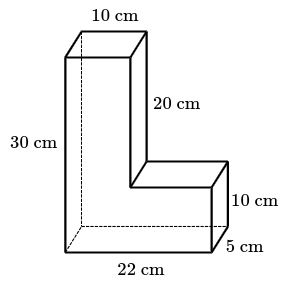
\includegraphics[width=0.75\textwidth]{../images/vol_area_02}
        \end{center}
        \caption{}
        \label{fig:vol_area_02}
    \end{figure}
\end{minipage}
\begin{minipage}{0.7\linewidth}
    \begin{solutionbox}{5cm}
    \end{solutionbox}
\end{minipage}